%X TS-program = pdflatex
% !TEX encoding = UTF-8 Unicode

% This is a simple template for a LaTeX document using the "article" class.
% See "book", "report", "letter" for other types of document.

\documentclass[oneside]{book} % use larger type; default would be 10pt
\usepackage{color}
\usepackage[utf8]{inputenc} % set input encoding (not needed with XeLaTeX)

%%% Examples of Article customizations
% These packages are optional, depending whether you want the features they provide.
% See the LaTeX Companion or other references for full information.

%%% PAGE DIMENSIONS

%\usepackage[top=20mm,right=20mm,bottom=15mm,left=20mm]{geometry}
% \geometry{margins=2in} % for example, change the margins to 2 inches all round
% \geometry{landscape} % set up the page for landscape
%   read geometry.pdf for detailed page layout information

\usepackage{graphicx} % support the \includegraphics command and options

% \usepackage[parfill]{parskip} % Activate to begin paragraphs with an empty line rather than an indent

%%% PACKAGES
\usepackage{booktabs} % for much better looking tables
\usepackage{array} % for better arrays (eg matrices) in maths
%\usepackage{paralist} % very flexible & customisable lists (eg. enumerate/itemize, etc.)

%\usepackage{subfig} % make it possible to include more than one captioned figure/table in a single float
\usepackage{amsfonts}
\usepackage{amsthm}
\usepackage{tikz}
\usepackage{amsmath}
\usepackage{float}
\usepackage{graphicx}
\usepackage{caption}
\usepackage{subcaption}
\usepackage{color}
\usepackage{amssymb}
\usepackage{bm}

% These packages are all incorporated in the memoir class to one degree or another...

%%% HEADERS & FOOTERS
\usepackage{fancyhdr} % This should be set AFTER setting up the page geometry
\pagestyle{fancy} % options: empty , plain , fancy
\renewcommand{\headrulewidth}{0pt} % customise the layout...
\lhead{}\chead{}\rhead{}
\lfoot{}\cfoot{\thepage}\rfoot{}

%%% SECTION TITLE APPEARANCE
%\usepackage{sectsty}
%\allsectionsfont{\sffamily\mdseries\upshape} % (See the fntguide.pdf for font help)
% (This matches ConTeXt defaults)

%%% ToC (table of contents) APPEARANCE
%\usepackage[nottoc,notlof,notlot]{tocbibind} % Put the bibliography in the ToC
%\usepackage[titles,subfigure]{tocloft} % Alter the style of the Table of Contents
%\renewcommand{\cftsecfont}{\rmfamily\mdseries\upshape}
%\renewcommand{\cftsecpagefont}{\rmfamily\mdseries\upshape} % No bold!


\newtheorem{theorem}{Theorem} 
\newtheorem{lemma}{Lemma}
\newtheorem{propn}{Proposition}
\newtheorem*{thmm}{Theorem}
\newtheorem{remk}{Remark} 
\newtheorem{corol}{Corollary}
\newtheorem{definition}{Definition}



\newtheorem{thm}{Theorem}[section] 
\newtheorem{prop}[thm]{Proposition} 
\newtheorem{lem}[thm]{Lemma}
\newtheorem{cor}[thm]{Corollary} 
\newtheorem{con}[thm]{Conjecture} 

\theoremstyle{definition}
\newtheorem{defn}[thm]{Definition}
\newtheorem*{rem}{Remark}
%\newtheorem*{nota}{Notation}
\newtheorem*{nota}{Notation}
\newtheorem{cla}[thm]{Claim}
\newtheorem{ex}[thm]{Example}
\newtheorem{exs}[thm]{Examples}
\newtheorem*{exer}{Exercise}
\newtheorem{case}{Case}
\newtheorem{conj}{Conjecture}
\numberwithin{equation}{section} 

\definecolor{sotonblue}{rgb}{0.0,0.394,0.597}

%\newcommand{\pspace}{$(\Omega_\alpha,\mathcal{F}_\alpha,P_\alpha)$ } 
\DeclareMathOperator{\Aut}{Aut} %Notation for automorphism group
%\DeclareMathOperator{\Pspace}{(\Omega, \mathcal{F},\mathbb{P})}
%\DeclareMathOperator{\Pspacen}{(\Omega_n, \mathcal{F}_n,\mathbb{P}_n)}

\DeclareMathOperator{\T}{\mathcal{T}}
\DeclareMathOperator{\lT}{\tilde{\mathcal{T}}_n}

\DeclareMathOperator{\N}{\mathbb{N}}
\DeclareMathOperator{\Pruf}{\mathcal{P}} %the space of prufer sequences
\DeclareMathOperator{\B}{\mathcal{B}}
\DeclareMathOperator{\F}{\mathcal{F}}
\DeclareMathOperator{\fix}{fix}

%opening
 \title{18 Month Report}
\author{David Matthews}
\begin{document}
\tableofcontents
\chapter*{\centering Abstract}\label{sec:intro}
\addcontentsline{toc}{chapter}{Abstract}
\begin{quotation}
 ``Perhaps an Erdos quote linking probability and graph theory'' 
\end{quotation}
A \emph{random recursive tree} is a finite nested family of labelled trees, $\{T_t\}_{t=1}^{n}$ built by iteratively attaching
a new vertex to one of the existing vertices uniformly at random. At step $t$ in this iteration let
$a_t = \lvert \Aut(T_t) \rvert$ where $\Aut(T_t)$ is the group of automorphisms of tree $T_t$.  MacArthur, (\cite{Bens}, Personal Communication), performed numerical calculations which suggest that in the limit $t \rightarrow \infty$
\[(a_t)^\frac{1}{t} \rightarrow \mathcal{V} \]
where $\mathcal{V}$ is an unknown constant redolent of the Fibonacci sequence.

A random Fibonacci sequence is a simple variation of the usual Fibonaci sequence in which $F(1) = F(2) = 1$ and $F$ is recursively defined for $n>2$:
\[F(n) = F(n-1) \pm F(n-2), \]
where the addition and negation are chosen equiprobably.  Viswanath \cite{Viswanath} showed that almost surely 
$|f(t)|^{\frac{1}{t}} \rightarrow 1.13198824 $ (a number that has subsequently become known as Viswanath's constant) as 
$t\rightarrow\infty$ although his proof was computational in nature \footnote{More recently Viswanath's constant was calculated to another 5 decimal places \cite{oli}}.   Macarthur made the following conjecture.

\begin{con}\label{conj:1}
In the limit $t \rightarrow \infty, a_t^\frac{1}{t} \rightarrow \mathcal{V} $ where $\mathcal{V}$ is Viswinath's constant.  
\end{con}

The primary goal of this project is to prove Conjecture \ref{conj:1}.
   
\chapter{Introduction}\label{sec:background}
\section{Attachment trees}\label{sec:att}
The set of vertices and the set of edges of some tree $T$ are denoted $V(T)$ and $E(T)$ respectively.  
A \emph{random attachment tree}, $T = \{T_t\}_{t=1}^n$ on $n$ vertices is a nested sequence of  labelled, rooted trees:
\[T_{1} \subset T_{2} \subset \dots \subset T_{n}.\]
Tree $T_{1}$ consists of 1 vertex and no edges. At subsequent time $t = 2,3,\dots,n$ a vertex, $v$, is chosen from 
$V(T_{t-1})$ according to some attachment model and a new vertex labelled $t$ is attached to $v$ via an edge. 

Note that each $T_i$ is indeed a tree since it has $i$ vertices and $i-1$ edges and each $T_i$ is obviously connected. 

If the attachment model is uniform random attachment then we say that $\{T_t\}_{t=1}^{n}$ is a \emph{ 
random recursive tree} on $n$ vertices. For succinctness we will henceforth refer to a random recursive trees as a RRT.  A random recursive $d$-ary tree is an attachment tree withe following attachment model.  The probability of a new vertex is uniformly distributed amongst the vertices with degree less than $d$ hence the proabbility of attaching to an existing vertex with degree $d$ is 0.   
\begin{figure}[ht]
\centering
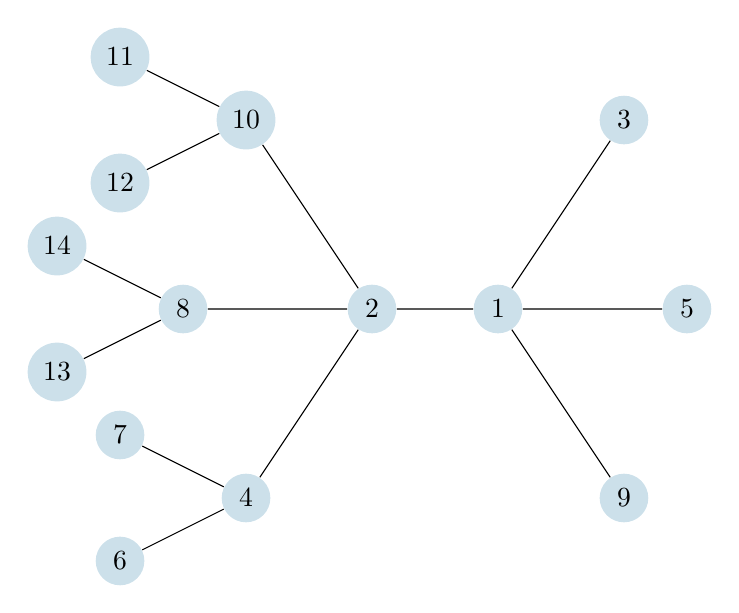
\begin{tikzpicture}
  [scale=0.8,auto=left,every node/.style={circle,fill=sotonblue!20}]

  \node (n1) at (7,5) {1};
  \node (n2) at (5,5)  {2};
  \node (n3) at (9,8)  {3};
  \node (n4) at (3,2) {4};
  \node (n5) at (10,5)  {5};
  \node (n6) at (1,1)  {6};
  \node (n7) at (1,3)  {7};
  \node (n8) at (2,5)  {8};
  \node (n9) at (9,2)  {9};
  \node (n10) at (3,8)  {10};
  \node (n11) at (1,9)  {11};
  \node (n12) at (1,7)  {12};
  \node (n13) at (0,4)  {13};
  \node (n14) at (0,6)  {14};
  \foreach \from/\to in {n1/n2,n1/n3,n1/n5,n1/n9,n2/n4,n2/n8,n2/n10,n10/n11,n10/n12,n8/n14,n8/n13,n4/n7,n4/n6}
    \draw (\from) -- (\to);
\end{tikzpicture}
\caption{An example of an attachment tree $T = \{T_t\}_{t=1}^{14}$.}\label{fig1}
\end{figure}

For any tree $T$ let  $d(v,w)$ be the length of the (unique) shortest path between any pair of vertices $v,w \in V(T)$. 
Each vertex (apart from 1) of an attachment tree is adjacent to precisely one vertex with a lower label. Furthermore, we 
define the \emph{father} of each vertex $v$ to be the vertex $v'$ adjacent to $v$ such that $d(v',1)< d(v,1)$. By the attachment 
process the father of a vertex is unique hence well-defined.

For example, consider the attachment tree $T$ in Figure \ref{fig1}, the distance $d(1,10) = 2$ and the father of vertex 13 is vertex 8.

\section{The automorphism group of labelled trees}\label{sec:yo}
%Definition - labelled tree?????
Two labelled trees $T_{1}$ and $T_2$ are considered the same and called isomorphic if and only if there is a 1-1 map $\alpha: V(T_1) \rightarrow V(T_2)$ which preserves adjacency and the labelling.  If $T_1 = T_2$ then $\alpha$ is called an automorphism.  The collection of all automorphisms of tree $T$ is  denoted $\Aut(T)$ and constitutes a group.

We denote the symmetric group on $n$ objects by $S_n$ and the set of all labelled trees by $\lT$.  We can act on $\lT$ with $S_n$ by permuting vertices i.e. for some $\sigma \in S_n$ and $T \in \lT$ we define $\sigma \cdot T$ to be the tree $T'$ such that $(\sigma(v),\sigma(w))$ is an edge of $T'$ if and only if $(v,w)$ is an edge of $T$.  We will abuse notation by writing $\sigma \in \Aut(T)$ if $\sigma \cdot T = T$.  

\begin{figure}[ht]
\centering
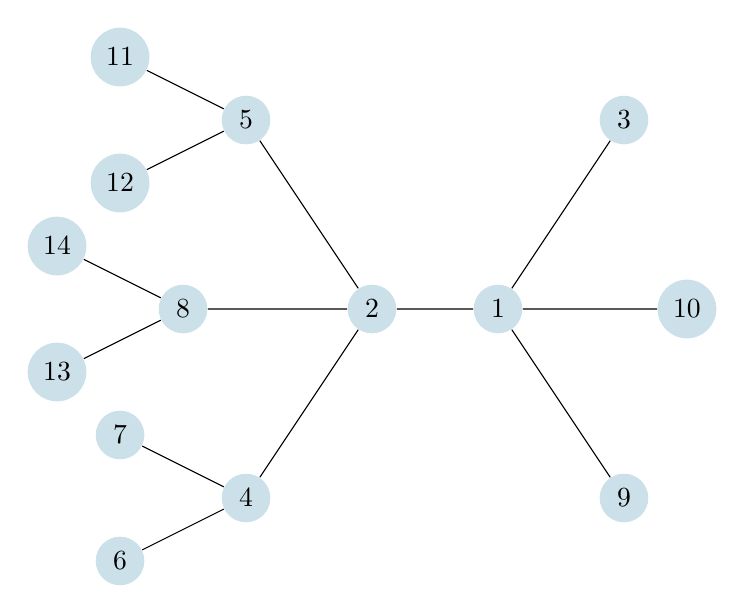
\begin{tikzpicture}
  [scale=0.8,auto=left,every node/.style={circle,fill=sotonblue!20}]

  \node (n1) at (7,5) {1};
  \node (n2) at (5,5)  {2};
  \node (n3) at (9,8)  {3};
  \node (n4) at (3,2) {4};
  \node (n5) at (10,5)  {10};
  \node (n6) at (1,1)  {6};
  \node (n7) at (1,3)  {7};
  \node (n8) at (2,5)  {8};
  \node (n9) at (9,2)  {9};
  \node (n10) at (3,8)  {5};
  \node (n11) at (1,9)  {11};
  \node (n12) at (1,7)  {12};
  \node (n13) at (0,4)  {13};
  \node (n14) at (0,6)  {14};
  \foreach \from/\to in {n1/n2,n1/n3,n1/n5,n1/n9,n2/n4,n2/n8,n2/n10,n10/n11,n10/n12,n8/n14,n8/n13,n4/n7,n4/n6}
    \draw (\from) -- (\to);
\end{tikzpicture}
\caption{This the tree $\sigma \cdot T$ where $\sigma$ is the transposition $(5,10)$ and $T$ is the tree in Figure \ref{fig1}.  Note that $\sigma$ is \emph{not} an automorphism of $T$.  }\label{fig15}
\end{figure}  
The orbits of this action are the unlabelled trees on $n$ vertices.  Denote the number of unlabelled trees on $n$ vertices by $t_n$ then by Burnside's lemma:
\begin{equation}\label{eqn:burnside}
   t_n = \frac{1}{\lvert S_n \rvert}\sum_{\sigma \in S_n} \lvert \fix(\sigma) \rvert
\end{equation}

Fix a permutation, $\sigma \in S_n$, and consider $\fix(\sigma) = \{T \in \lT : \sigma \cdot T  = T\}$. The permutation $\sigma \in \Aut(T)$ for all $T \in \fix(\sigma)$.  To make this clear consider the indicator function:
\[
 I(\sigma,T) = \begin{cases}
                1 & \text{if}\ \sigma \in \Aut(T) \\
                0 & \text{otherwise.}
               \end{cases}
\]

The expected order of automorphism group of a labelled tree on $n$ vertices is:
\begin{align}
\mathbb{E}(\Aut_n(T)) &= \frac{1}{\lvert \lT \rvert}\sum_{T \in \lT} \lvert \Aut(T) \rvert \\
&= \frac{1}{\lvert \lT \rvert}\sum_{\sigma \in S_n}\sum_{T \in \lT} I(\sigma,T) \\
&=  \frac{1}{\lvert \lT \rvert}\sum_{\sigma \in S_n}\lvert \fix(\sigma) \rvert \\
&= \frac{t_n\lvert S_n\rvert}{\lvert \lT \rvert}.
\end{align}


\section{Automorphisms of random recursive trees}\label{sec:aorrt}
 It is a result of P\'{o}lya that the automorphism group of a tree belongs to the class of permutation groups which contains the symmetric groups and is closed under taking direct and wreath products \cite{biggs:1993}. Therefore there exists a direct product decomposition for any tree $T$:
 \begin{equation}\label{decomp}
  \Aut(T) \cong A_{1} \times A_{2} \times\dots\times A_{p} \times B_{1} \times B_{2} \times \dots \times B_{q}
 \end{equation}
Such that $A_{i} \cong S_{x(i)}$ and $B_{j} = S_{y_{1}(j)} \wr S_{y_{2}(j)} \wr \dots \wr S_{y_{k_{j}}(j)}$.

In addition to this algebraic interpretation of $\Aut(T_{n})$ there is a pleasing geometric realisation of equation \ref{decomp}.  In this geometric realisation each symmetric factor $S_k$ corresponds to a hub vertex adjacent to $k$ paths of length $n$, each of which terminates in a leaf. Each wreath product factor, $B_{i}$, corresponds to an extended symmetric induced subtree \cite{Ben}. We denote an induced subtree consisting of a hub vertex adjacent to $k$ paths of length $n$ a $(n,k)$-star.  For succinctness we will refer to $(1,k)$-stars simply as $k$-stars.  These $(n,k)$-stars and extended symmetric branches are known as \emph{network motifs} and have been described as the building blocks of many real-world networks \cite{milo}.

\begin{figure}[ht]
\centering
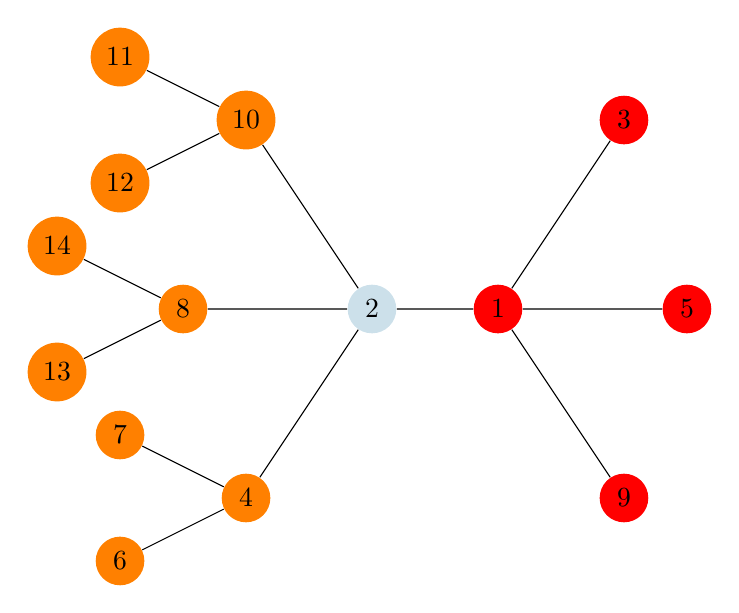
\begin{tikzpicture}
  [scale=0.8,auto=left,every node/.style={circle,fill=sotonblue!20}]

  \node[style={circle,fill=red!100}] (n1) at (7,5) {1};
  \node (n2) at (5,5)  {2};
  \node[style={circle,fill=red!100}] (n3) at (9,8)  {3};
  \node[style={circle,fill=orange!100}] (n4) at (3,2) {4};
  \node[style={circle,fill=red!100}] (n5) at (10,5)  {5};
  \node[style={circle,fill=orange!100}] (n6) at (1,1)  {6};
  \node[style={circle,fill=orange!100}] (n7) at (1,3)  {7};
  \node[style={circle,fill=orange!100}] (n8) at (2,5)  {8};
  \node[style={circle,fill=red!100}] (n9) at (9,2)  {9};considering
  \node[style={circle,fill=orange!100}] (n10) at (3,8)  {10};
  \node[style={circle,fill=orange!100}] (n11) at (1,9)  {11};
  \node[style={circle,fill=orange!100}] (n12) at (1,7)  {12};
  \node[style={circle,fill=orange!100}] (n13) at (0,4)  {13};
  \node[style={circle,fill=orange!100}] (n14) at (0,6)  {14};
  \foreach \from/\to in {n1/n2,n1/n3,n1/n5,n1/n9,n2/n4,n2/n8,n2/n10,n10/n11,n10/n12,n8/n14,n8/n13,n4/n7,n4/n6}
    \draw (\from) -- (\to);
\end{tikzpicture}
\caption{An example of a random recursive tree, $T$, such that $\Aut(T) \cong S_{3} \times S_{2}\wr S_{3}$.  
The red vertices indicate an induced subtree $\tilde{T}_{v_{1}}$ isomorphic to the bipartite graph $k_{1,3}$ which 
contributes $S_{3}$ to $\Aut(T_{14})$. The orange nodes highlight an induced subtree, $\tilde{T}_{v_{2}}$ of $T_{14}$ 
isomorphic to an extended symmetric subtree and contributes $S_{2}\wr S_{3}$ to $\Aut(T)$.}\label{fig2}
\end{figure}

Let $T$ be a tree.  There is a natural way to split $\Aut(T)= A_{1} \times\dots\times A_{p} \times B_{1} \times \dots \times B_{q}$ into two subgroups.  The direct product of symmetric groups form the \emph{elementary subgroup}:
\[
 \mathcal{E}(T) = A_{1} \times A_2 \times \dots\times A_{p}
\]
The direct product of wreath products of symmetric groups form the \emph{complex subgroup}:
\[
 \mathcal{C}(T) =  B_{1} \times B_2 \times \dots \times B_{q}
\]
The elementary subgroup captures the contribution that $(n,k)$-stars make to the automorphism group and the complex subgroup captures the contribution that the extended symmetric branches make to the automorphism group.  The order of the automorphism group of tree $T$ can also be split as follows:
\[
\lvert \Aut(T) \rvert  =  \lvert \mathcal{E}(T) \rvert\lvert \mathcal{C}(T)\rvert 
\]
This begs the question: does the order of either the elementary or the complex subgroup dominate the other?  MacArthur \cite{Bens} made the following additional conjecture:
\begin{con}\label{conj:2}
 Let $\{T_t\}_{t=1}^{n}$ be a RRT. In the limit as $n \rightarrow \infty$, $\lvert \mathcal{E}(T_n)\rvert^{\frac{1}{n}}  = \mathcal{V}$, while in the limit as $n \rightarrow \infty$, $\lvert \mathcal{C}(T_n)\rvert^{\frac{1}{n}}  = 1$.
 
 \end{con}
If conjecture \ref{conj:2} were true then to prove conjecture \ref{conj:1} it is enough to calculate the limiting behaviour of $(n,k)$-stars.  

In Chater \ref{sec:Prufer} we refine a bijection of Pr\"{u}fer between labelled trees on $n$ vertices and sequences called Pr\"{u}fer
 sequences by restricting this bijection to random recursive trees.  As a result there is an obvious way to give the set $\T_n$ 
 additional structure by thinking it as a topological and then a measure space.
 
In Chapter \ref{chap:Joyal} we exploit another bijection, this time between $\T_n$ and a certain class of integer valued 
functions.  We define what it is to be an automorphism of these functions and use a varaiant of equation \ref{} to calculate the 
expected number of $k$-stars in a random recursive tree on $n$ vertices.

In Chapter \ref{chap:perms} we construct several further bijections between $\T_n$ and a class of binary trees, and a set of 
recursively defined permutations via a combinatorial setup known as a Chinese Restraunt Process.  We show that many of the results 
from the theory of random permutations can be fruitfully applied to RRTs.  For example, we calculate the expected number of leaves in
a RRT on $n$ vertices. We conclude Chapter \ref{chap:perms} by suggesting a possible future path in order to calculate the
expected number of $(k)$-stars in a RRT. 

Finally, in Chapter \ref{chap:polya} we build a statistical device called a Polya Urn scheme to output the features of a typical 
RRT such as the degree distribution, the number of $(n,k)$-stars and the number of extended symmetric branches.  We then give limits
 for the order of limiting order of the elementary subgroup $\lvert \mathcal{E}(T) \rvert$.  We end Chapter \ref{chap:polya}  by 
 proving that conjecture \ref{conj:2} is false. 

%Definition of un/rooted, un/labelled trees
\chapter{A Measure on Random Recursive Trees}

\section{Pr\"{ufer} sequences}\label{sec:Prufer}

Cayley was first to prove that there are $n^{n-2}$ labelled trees on $n$ vertices \cite{Cayley}. A later proof due 
to Pr\"{u}fer uses a correspondence between particular sequences called \emph{Pr\"{u}fer sequences} and labelled trees 
\cite{Bela}.  

Let the set of the first $n$ integers be denoted $\N_n = \{1,2,3,\dots n\}$.  A Pr\"{u}fer sequence $P_n = (a[1],a[2],\dots a[n-2])$
is a sequence of length $n-2$ where each entry $a[i]\in \N_n$. For example $P = (2,1,4,5,4,2,2,2,5,7,7)$ is a Pr\"{u}fer sequence. 

If $A$ and $B$ are sets, we denote the set of elements in $A$ and not in $B$ by $A \backslash B$. Let $L(P_n)$ be the set of all elements $l \in P_n \backslash \N_n$.  For example, $L(P) := \{3,6,8,9,10,11,12,13\}$.

The set of Pr\"{u}fer sequences of length $n-2$ is denoted $\Pruf_n$.  Pr\"{u}fer showed that there exists the following bijection. 
\[
  f: \Pruf_n \rightarrow\tilde{\T}_n 
\]
via the following dynamic correspondence.  Let $P_n = (a[1],a[2],\dots a[n-2])$ be a Pr\"{u}fer sequence.
\begin{itemize}
 \item[(i)] At time $t=0$ define graph $G_0$ to have $n$  vertices and no edges and  define $L_0 = L(P_n)$. 
 \item[(ii)] At times $t=1,2,\dots, n-2$ construct $G_t$ from $G_{t-1}$  by adding the edge $(a[t],\min(L_{t-1})$ and the set $L_t$
 is build from $L_{t-1}$ by removing element $\min(L_{t-1})$ and, if for all $i$ such that $a[i] = a[t]$, $i \leq t$ $a[t]$ then add $a[t]$ to $L_{t-1}$.
 \item[(iii)]Let $D$ be the number of distinct entries of $P_{n}$. Since $D$ elements are added to $L_{0}$ and $n-2$ elements are removed
to form $L_{t-1}$:
\[|L_{n-1}| = |L_{0}| + D - (n-2).\]
Therefore $|L_{n-1}| = 2$. Finally, $G_{n-1}$ is formed by adding an edge between the two vertices in $ 
L_{n-1}$.
\end{itemize}
Graph $G_{n-1}$ consists of $n$ vertices and $n-1$ edges.  Since for every $x \in \N_{n}$ there exists an $i$ such that $x \in L_i$ every vertex in $G_{n-1}$ is incident to at least one edge so $G_{n-1} \in \tilde{\T_n}$.  

Given a labelled tree $T_n$ we can generate a Pr\"{u}fer sequence by removing the smallest leaf of $T_n$ at time $i$ and assigning $a[i]$ to be the vertex adjacent to $i$ for $i = 1,2,\dots,n-2$. For example $P = (1,1,4,4,2,1,2,10,10,2,8,8)$ is the unique Pr\"{u}fer sequence that corresponds to tree $T$ in Figure \ref{fig1}. Map  $f$ is a bijection and as a corollary:
\[
 \lvert \tilde{\T_n} \rvert  = \lvert \Pruf_n \rvert  = n^{n-2} 
\]

We could restrict $f^{-1}$ to RRTs as $f^{-1} |_{\T_n}: \T_n \rightarrow \Pruf_n$ and ask the question: what form does the image of $f^{-1} |_{\T_n}$ take? 

Define another bijection $f^{*}: \P_n \rightarrow \lT$ via a similar correspondence to map $f$.  We define $L$ and $G_0$ as before and at times $t=1,2,\dots n-2$ we construct $G_t$ from $G_{t-1}$ by adding the edge $(a[t],\max(L_{t-1})$.  We can uniquely construct the preimage of labelled tree $T \in \lT$ by removing the leaf with the largest label and setting $a[1]$ to be the vertex adjacent to that leaf. Entry $a[2]$ is the vertex attached to the new greatest value leaf and so on.  For example, the Pr\"{u}fer sequence that corresponds to $T$ in Figure \ref{fig1} under $f^*$ is:
\[P = (8,8,10,10,2,1,2,4,4,1,2,1).\]
If $T\in \T_n$ then $a[1]$ is the father of vertex $n$, entry $a[2]$ is the father of $n-1$ and in general $a[i]$ is the father of vertex $n + 1-i$ in the corresponding Pr\"{u}fer sequence.
\begin{cor}
 Pr\"{u}fer sequence $P = (a[1],a[2],\dots,a[n-2])$ corresponds to a RRT $T \in T_n$ if and only if $a[i] \in \N_{n-i}$ 
\end{cor}

\begin{cor}
\[
 \lvert T_n \rvert  = (n-1)!
\]
\end{cor}
Note that $a[i]$ corresponds to the father of node $n-i$ in $T_n$ and as therefore $L$ is the set of leaves of $T_n$.  

\section{The space of random recursive trees}
By Section \ref{sec:Prufer} every RRT can be associated with a unique nested set of Pr\"{u}fer sequences:
\[P_{n-1} \supset P_{n-2} \supset \dots \supset P_3\]
where each $P_3 = (a[1])$ with $a[1] \in \N_2$ and subsequent $P_i$ are built from $P_{i-1}$ by the addition of $a[i-2] \in \N_{i}$.  In fact $a[i]$ is the father of vertex $i+2$ for $i = 1,2,\dots, n-2$.  The set, $\T_n$, of all RRTs on $n$ vertices can be considered as the set $\Pruf_n$ of all nested  of Pr\"{u}fer sequences of length $n$.  We can make $\Pruf_n$ a topological product space,
\[
 \Pruf_n = \prod_{i=2}^{n-1} \N_i,
\]
where each $\N_i$ is equipt with the discrete topology.  We can further define a measure on $\Pruf_n$ by appealing to the following Theorem of Tao \cite{Tao}:
\begin{theorem}\label{thm:tao}

 Let $A$ be an arbitrary set.  For each $\alpha \in A$ let $(\Omega_{\alpha},\mathcal{F}_\alpha,P_\alpha)$ be a probability space such that $\Omega_{\alpha}$ is a locally compact, $\sigma$-compact metric space with Borel $\sigma$-algebra $\mathcal{F}_{\alpha}$ then there exists a unique probability measure
 \[
  P_{A} = \prod_{\alpha \in A}P_\alpha \text{   on   } \left(\prod_{\alpha \in A}\Omega_\alpha, \prod_{\alpha \in A}\mathcal{F}_\alpha,\right)  
 \]
 Such that $P_A\left(\prod_{\alpha \in A}E_\alpha\right)  = \prod_{\alpha \in A} P_\alpha(E_\alpha)$.  
 
 Furthermore, whenever $E_\alpha \in \mathcal{F}_\alpha$ one has $E_\alpha = \Omega_{\alpha}$ for all but finitely many $\alpha$. 
\end{theorem}

\begin{cor}
 There exists a unique measure $\mu$ on $\Pruf_n$. 
\end{cor}

\begin{proof}
 Let $A = \N_n$, then for each $\alpha \in \N_n$ let $X_\alpha = \N_{\alpha}$ with the discrete metric (and the discrete $\sigma$-algebra) and the uniform probability measure $\mu_{\alpha}$ in the statement of Theorem \ref{thm:tao}.   
\end{proof}

For each $i \in \N_\alpha$ we have coordinate projection maps $\pi_{i} : \Pruf_n \rightarrow \N_i$ defined by $\pi_1(P_n):= 1$ and $\pi_i(P_n):= a[i]$ for $i = 2,3\dots,n-1$.  Therefore a RRT can be interpreted as a sequence of random variables taking values in $\N_{\alpha}$ for $\alpha  = 1,2,\dots n-1$.  The measure $P_{\N_n}$ is a uniform probability measure on $\T_n$.   

\chapter{Random Recursive Trees as Functions}\label{chap:Joyal}
Let $\mathcal{F}_n$ be the set of functions $f: \N_n \longrightarrow \N_n$ such that $f(1) = 1$ and $f(i) <i$ for $i = 2,3,\dots n$.

\begin{lem}
  There is a bijection, $\alpha: \T_n \rightarrow \mathcal{F}_n$.
\end{lem}

\begin{proof}  Let $T = \{T_t\}_{t=1}^n$ be a RRT on $n$ vertices.  Construct $\alpha(T)$ by assigning $f(1) = 1$ and $f(i)$ 
to be the father of vertex $i$ for $i = 2,3,\dots n$. On the other hand consider a function $f \in \F_n$; we construct the
preimage under $\alpha$ of $f$ as follows. Let $T_1$ be the tree on 1 vertex and 0 edges and build tree $T_i$ from $T_{i-1}$ by attaching vertex $i$ to vertex $f(i)$ via an edge. This preimage is clearly unique, therefore $\alpha$ is a bijection.     
\end{proof}

\begin{cor}
$\lvert \T_n \rvert =  (n-1)!$
\end{cor}
\begin{proof}
 Since $\lvert \T_n \rvert = \lvert \mathcal{F}_n \rvert$ it is enough to enumerate $\mathcal{F}_n$.  
Given any function $f \in \F_n$ by definition $f(i) \in \N_{i-1}$ for $i= 2,3,\dots,n$.  We can think of this as 1 choice for $f(2)$, 
2 choices for $f(3)$ and in general $i-1$ possible choices for $f(i)$.  
\[ \lvert \mathcal{F}_n \rvert = (n-1)!\]
\end{proof}


%Section on Joyal - action on joyal via a permutation.


\section{Expected automorphism group of a random recursive trees}
In Section \ref{sec:yo} we noted that the expected order of automorphism group of a labelled tree on could be calculated via
the action of $S_n$ on $\lT$ and applying Burnside's Lemma.  This begs the question: is it possible to build a similar argument for the space of RRTs? 

There does not exist an analogous group action of $S_n$ on $\T_n$. For example, let $T$ be the RRT shown in Figure \ref{fig1}.
If we forget that $T$ is a RRT and think of $T$ as a labelled tree we can act $T$ with $S_n$.  The action of the 
transposition $(1,5)$ on $T$ is shown in Figure \ref{fig3} and is \emph{not} a RRT since vertex 5 is attached to 3 vertices with smaller labels. 

\begin{figure}[ht]
\centering
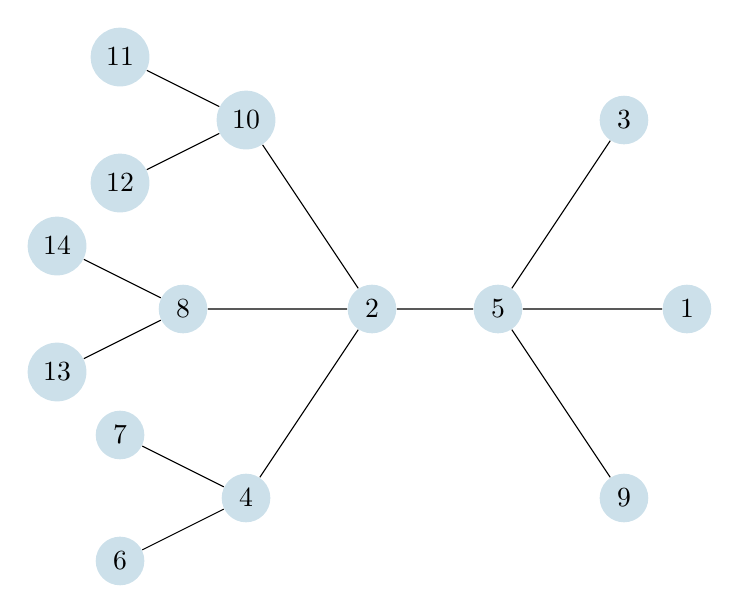
\begin{tikzpicture}
  [scale=0.8,auto=left,every node/.style={circle,fill=sotonblue!20}]

  \node (n1) at (7,5) {5};
  \node (n2) at (5,5)  {2};
  \node (n3) at (9,8)  {3};
  \node (n4) at (3,2) {4};
  \node (n5) at (10,5)  {1};
  \node (n6) at (1,1)  {6};
  \node (n7) at (1,3)  {7};
  \node (n8) at (2,5)  {8};
  \node (n9) at (9,2)  {9};
  \node (n10) at (3,8)  {10};
  \node (n11) at (1,9)  {11};
  \node (n12) at (1,7)  {12};
  \node (n13) at (0,4)  {13};
  \node (n14) at (0,6)  {14};
  \foreach \from/\to in {n1/n2,n1/n3,n1/n5,n1/n9,n2/n4,n2/n8,n2/n10,n10/n11,n10/n12,n8/n14,n8/n13,n4/n7,n4/n6}
    \draw (\from) -- (\to);
\end{tikzpicture}
\caption{Tree $(1,5) \cdot T$}\label{fig3}
\end{figure}

Even though $S_n$ does not act on $\T_n$ we can define $\sigma \cdot T$ to be the tree such that $(\sigma(v),\sigma(w)) \in E(\sigma \cdot T)$ if and only if $(v,w) \in E(T)$.  If $\sigma \cdot T \in \T_n$ then there exists a function $f' \in \F_n$ corresponding to $\sigma \cdot T$.  We describe the precise form of $f'$ in Lemma \ref{fdash}. 

\begin{lem}\ref{lem:fdash}
Let $T \in T_n$ correspond to $f \in \mathcal{F}_n$ and  $\sigma \cdot T \in \Aut(T)$ correspond to function $f' \in \F_n$, then $f_n$ has the following form:  
\[ f'= \left(\begin{array}{cccccc}
     1& \sigma(2)&\sigma(3) &\sigma(4)& \dots & \sigma(n) \\
     1 & \sigma(f(2)) &\sigma(f(3)) &\sigma(f(4)) &\dots & \sigma(f(n))
    \end{array} \right)
\]
\end{lem}

\begin{proof}
 Let $T' = \sigma \cdot T$, there exists some function $g$ corresponding to $T'$ such that:
 \[ g= \left(\begin{array}{cccccc}
     1& \sigma(2)&\sigma(3) &\sigma(4)& \dots & \sigma(n) \\
     1 & g(\sigma(2)) &g(\sigma(3)) &g(\sigma(4)) &\dots & g(\sigma(n))
    \end{array} \right)
\]

Where $g(\sigma(i))$ is the father of $\sigma(i)$ but it is clear that the father of $\sigma(i)$ is $\sigma(f(i))$  hence $g(i) = \sigma(f(i))$ for $i = 2,3,\dots,n$.  
\end{proof}

\begin{cor}\label{cor:sig}
Let $T \in \T_n$ and $ \sigma \in S_n$.  Then  $\sigma  \cdot T \in \T_n$ if and only if $\sigma(f(i)) < \sigma(i) $. 
\end{cor}

%D%escribe bijections between RRTs and prufer sequences/joyal functions.

Let $T \in T_n$. $\sigma \in S_n$ and recall the definition of the indicator function from Section \ref{sec:yo}:
\[
 I(\sigma,T) = \begin{cases}
                1 & \text{if}\ \sigma \in \Aut(T) \\
                0 & \text{otherwise.}
               \end{cases}
\]
The expected size of the automorphism group of a RRT is:
\begin{align}
 \frac{1}{\lvert\T_n\rvert}\sum_{T \in \T_n} \lvert \Aut(T) \rvert &=  \frac{1}{\lvert\T_n\rvert}\sum_{T \in \T_n}\sum_{\sigma \in S_n}I(\sigma,T) \\
 &=   \frac{1}{\lvert\T_n\rvert}\sum_{\sigma \in S_n}\sum_{T \in T_n}I(\sigma,T) \\
\end{align}
For each permutation $\sigma \in S_n$ we define:
\[
 J(\sigma) = \frac{1}{\lvert \T_n \rvert}I(\sigma,T)
\]
In this section we will calculate $J(\sigma)$ when $\sigma = (p_1,p_2,\dots,p_m)$ is a cycle of length $1 \leq m<n$ with the additional condition $p_1< p_2<\dots< p_m$ .

\begin{remk}\label{remk:1}
 The geometric decomposition of the group of automorphisms of a tree discussed in section \ref{sec:aorrt} means that an
 automorphism $\sigma \in \Aut(T)$ corresponds to either an $(n,k)$-star or an extended symmetric branch of $T$.  In 
 particular, $\sigma = (p_1,p_2,\dots,p_m) \in \Aut(T)$ if and only if $p_1,\dots,p_m$ are the leaves of a $(1,m')$-star 
 in $T$ for some $m' > m$. Equivalently $\sigma \in \Aut(T)$ if and only if $f(p_1) = f(p_2) = \dots = f(p_m)$ and 
 $1 = \deg(p_1) = \deg(p_2) = \dots = \deg(p_m)$, where $f\in F_n$ is the unique function associated with $T$.   
\end{remk}

\begin{lem}\label{lem:2cycle}
 Consider the permutation $\sigma = (p_1,p_2) \in S_{n-1}$ such that without loss of generaity $p_1 < p_2$; then
 \[
  J(\sigma) = \frac{(p_1-1)}{(n-1)(n-2)}
 \]
\end{lem}
\begin{proof}
 By Lemma \ref{remk:1}, a permutation $\sigma \in \Aut(T)$ if and only if $f(p_1) = f(p_2)$ and $\deg(p_1) = \deg(p_2) = 1$.  Since every RRT $T \in T_n$ corresponds to a unique function $f \in F_n$ we can restate remark \ref{remk:1} as follows:  permutation $\sigma \in Aut(T)$ if and only if $f(p_1) = f(p_2)$ and $p_1,p_2$ are \emph{not} contained in the image of $f$. 
 
Following the proof of Corollary \ref{cor:sig}, we can think of $f(i) \in \N_{i-1}$ for $i = 2,3,\dots,n$  as $i-1$ choices for each $i$.  The additional restriction that $f(p_1) = f(p_2)$ means that there is exactly one choice to make for $f(p_2)$.  The restriction that $p_1$,$p_2$ are not contained in the image of $f$ means that there is 1 less choice for $f(i)$ where $i >p_1$ (apart from the case $i=p_2)$) and 2 less choices for $f(i)$ when $i >p_2$.  The proportion of functions $f$ such that  that $\sigma \in \Aut(T)$ can be calculated with the aid of the following table:
 \begin{equation}\label{eqn:tab}  \left(\begin{array}{ccccccccc}
       \dots & p_1 & p_1 +1            & \dots & p_2-1               & p_2              & p_2+1               &\dots  & n \\
       \dots & 1   & \frac{p_1-1}{p_1} & \dots & \frac{p_2-3}{p_2-2} & \frac{1}{p_2 -1} & \frac{p_2 - 2}{p_2} & \dots & \frac{n-3}{n-1}
    \end{array} \right)
\end{equation}
      The second row of table \ref{eqn:tab} describes the proportion of functions $f$ that satisfy the aforementioned conditions for each $i \in 2,3,\dots, n$.  We can therefore read off the table:
 \begin{align}
 J(\sigma) &= \frac{(n-3)!(p_1-1)}{(p_1 - 2)(n-1)!}\\
 &= \frac{(p_1-1)}{(n-1)(n-2)}
 \end{align}
\end{proof}
The method of proof in Lemma \ref{lem:2cycle} can be generalised as follows:
\begin{lem}\label{lem:3cycle}
 Let $\sigma = (p_1,p_2,\dots,p_m) \in S_n$ such that $p_1 < p_2< \dots <p_m$, then:
 \[
 J(\sigma) = \frac{(p_1-1)(n-m-1)!}{(n-1)!}
 \]
\end{lem}
\begin{proof}
 Since each RRT, $T \in \T_n$ corresponds to a function $f\in \F_n$ we need only consider automorphisms of $\F_n$.  By Remark \ref{remk:1}, the permutation $\sigma \in \Aut(T)$ if and only if $f(p_1) = f(p_2) = \dots f(p_m)$ and $p_1,p_2,\dots,p_m$ are not contained in the image of the corresponding function $f$.  Following the proof of Lemma \ref{lem:2cycle}, consider the following table:
  \[
\label{eqn:tab}  \left(\begin{array}{ccccccccccccc}
       \dots & p_1 & p_1 +1            & \dots & p_2-1               & p_2              & p_2+1               & \dots & p_{m}-1                & p_m            &p_m+1 &\dots &   n\\
       \dots & 1   & \frac{p_1-1}{p_1} & \dots & \frac{p_2-3}{p_2-2} & \frac{1}{p_2 -1} & \frac{p_2 - 2}{p_2} & \dots & \frac{p_m - m-1}{p_m-2} & \frac{1}{p_m-1} & \frac{p_m-m}{p_m} &\dots  &  \frac{n-m-1}{n-1}
    \end{array} \right)
\]
Following the proof of Lemma \ref{lem:2cycle} we can read off the table to ascertain:
\begin{align}
 J(\sigma) &= \frac{(n-m-1)!(p_1-1)!}{(p_1-2)!(n-1)!}\\
 &= \frac{(n-m-1)!(p_1-1)}{(n-1)!}
\end{align}

 
\end{proof}


Let $H_n(m)$ be the subset of $S_n$ consisting of all permutations $\sigma = (p_1,p_2,\dots,p_m)$ such that $p_1 < p_2 <\dots < p_m$ and define the number of automorphisms coming from all such permutations as:
\[X_n(m) = \sum_ {\sigma \in H_n(m)}J(\sigma)\]

\begin{lem}\label{lem:xn2}
 $X_n(2) = \frac{n}{3!}$
\end{lem}
\begin{proof}
 We can usefully lay out all possible permutations $\sigma \in H_n(2)$ as follows:
  \[ \begin{array}{c|c|c|c|c}
     (2,3)  & (2,4)  & (2,5) & \dots & (2,n) \\
       & (3,4)  & (3,5) & \dots &(3,n) \\
       &        &  (4,5) & \dots & (4,n) \\
       &&&& \vdots \\
       &&&&(n-1,n)
    \end{array} 
\]
Summing over rows and then columns and applying Lemma \ref{lem:2cycle} we see that:
\begin{equation}\label{eqn:tri}
  X_n(2) = \frac{1}{(n-1)(n-2)}\sum_{i=1}^{n-2}i \sum_{j=1}^{n-i-1}1 = \frac{n}{6}
\end{equation}


\end{proof}
\begin{lem}\label{lem:xn3}
 $X_n(2) = \frac{n}{4!}$
\end{lem}
\begin{proof}
 We can usefully lay out all possible permutations $\sigma \in H_n(3)$ in $n-3$ ``triangles'' as follows:
  \[ \begin{array}{c|c|c|c|c}
     (2,3,4)  & (2,3,5)  & (2,3,6) & \dots & (2,3,n) \\
       & (2,4,5)  & (2,4,6) & \dots &(2,4,n) \\
       &        &  (2,5,6) & \dots & (2,5,n) \\
       
       &&&& \vdots \\
       &&&&(2,n-1,n) \\
       &&&& \\
       &(3,4,5) &(3,4,6)&\dots&(3,4,n)\\
       &&(3,5,6)&\dots&(3,5,n)\\
        \vdots & \vdots &  \vdots &  \vdots &  \vdots
    \end{array} 
\]
Note that all permutations in a triangle take the same value for $p_1$. Hence summing over each triangle and a simple application of Lemma \ref{lem:3cycle} gives us:
\begin{equation}\label{eqn:tet}
  X_n(2) = \frac{1}{(n-1)(n-2)(n-3)}\sum_{i=1}^{n-3}i \sum_{j=1}^{n-i-2}j = \frac{n}{4!}
\end{equation}


\end{proof}



We define the \emph{generalised triangular numbers} as follows: let $T^{(2)}_i = 1$ for $i = 1,2,3,\dots$, and define $T^{(m)}_{i} = \sum_{j=1}^iT_{j}^{2}$.  This means that $T^{(3)}$ are the natural numbers, $T^{(4)}$ are the triangular numbers, $T^{(5)}$ are the tetrahedral numbers and so on.  We can reformulate equations \ref{eqn:tri} and \ref{eqn:tet} as follows:
\begin{align}
 X_n(2) &=  \frac{1}{(n-1)(n-2)}\sum_{i=1}^{n-2}i\sum_{j=1}^{n-i-1} T^{(2)}_{j} \\
 X_n(3) &=  \frac{1}{(n-1)(n-2)(n-3)}\sum_{i=1}^{n-3}i \sum_{j=1}^{n-i-2} T^{(3)}_{j} 
\end{align}

Following the proofs of Lemma \ref{lem:xn2} and \ref{lem:xn3} we can think of all possible permutations $\sigma \in H_n(m)$ in $n-m$, ``$m-1$-simplicies'' such that each $m-1$-simplex has the same value of $p_1$. We use Lemma \ref{lem:3cycle} to get:
\begin{equation}
 X_n(m) = \frac{(n-m-1)!}{(n-1)!}\sum_{i=1}^{n-m} i \sum_{j=1}^{n-i-m+1}T^{(m)},
\end{equation}
for $m = 1,2,\dots n-1$.

In order to find a general form for $X_n(m)$ we will split it up into constituent parts $\frac{(n-m-1)!}{(n-1)!}$ (which we can calculate) and 
\begin{equation}\label{eqn:xdash}
 X'_n(m) = \sum_{i=1}^{n-m} i \sum_{j=1}^{n-i-m+1}T^{(m)}
\end{equation}
\begin{figure}

\subsection{Pascal's triangle: an aside}

\begin{tabular}{rccccccccc}
$n=0$:&    &    &    &    &  1\\\noalign{\smallskip\smallskip}
$n=1$:&    &    &    &  1 &    &  1\\\noalign{\smallskip\smallskip}
$n=2$:&    &    &  1 &    &  2 &    &  1\\\noalign{\smallskip\smallskip}
$n=3$:&    &  1 &    &  3 &    &  3 &    &  1\\\noalign{\smallskip\smallskip}
$n=4$:&  1 &    &  4 &    &  6 &    &  4 &    &  1\\\noalign{\smallskip\smallskip}
\end{tabular}
\caption{Pascal's Triangle}\label{fig:pt}
\end{figure}
To calculate $X'_n(m)$ we must make some preliminary definitions regarding binomial coefficients and, although the suject is 
extremely elementary, it is appropriate to discuss Pascal's triangle because it draws together many themes of this chapter.  
Pascal's triangle, is an array of binomial coefficients such that the rows are enumerated from $n=0$ at the top and the columns 
are enumerated from left to right beginning with $k=0$.  Row $n$ has $n+1$ columns and the entry in the $n^{th}$ row and $k^{th}$
column is:

\[
 {n \choose k} = \frac{n!}{(n-k)!k!}.
\]
The first 5 rows of Pascal's triangle are shown in figure \ref{fig:pt}.  Note that ${n chose k}$ is also the number of ways
(disregarding order) that $k$ objects can be chosen from among $n$ objects.  There is a deep connection between generalised
triangular numbers and binomial coefficients \cite{}. For example, reading diagonally downwards in either direction of Pascl's 
triangle are the sets $T^{(2)}, T^{(3)},T^{(4)}\dots$ and note that:
\begin{equation}\label{eq:cho}
 \sum_{i=1}^{n}T_i^{(m)} = {n + (m-2)\choose(m-1)}
\end{equation}
Finally, for the readers amusement, recall that summing the upward diagonals gives the Fibonacci sequence.

\section{Expected automorphism group of a random recursive tree continued}

By Equation \ref{eq:cho} we can rewrite equation \ref{eqn:xdash} as:
\[ X'_n(m) = \sum_{i=1}^{n-m} i  {n-1-i\choose m-1} \]


In order to prove Lemma \ref{lem:xdash} we will also need the following identity:
\begin{equation}\label{eqn:id1}
{{n}\choose{k}} = {{n-1}\choose{k-1}} + {{n-1}\choose{k}}
\end{equation}

\begin{lem}\label{lem:xdash}
 $X'_n(m) = {n\choose m+1}$ for $m = 2,3,\dots,n-1$
\end{lem}
\begin{proof}
 We will use induction on $n$.  For the base case consider $n=3$ and $m=2$.  
 \[X_3'(2) = \sum_{i=1}^{3-2} i {3-i-1\choose 1} = {1\choose 1} = 1 = {3\choose3}.
 \]
Assume $X'_n(m) = {n\choose m+1}$ for $m = 2,3,\dots,n-1$ and consider $X_{n+1}(m)$.  In the case that $m =n$,
\[ X_{n+1}'(n) = \sum_{i=1}^1 i {m-i\choose m-1}  = 1 = {m+1 \choose m+1}\]
On the other hand if $m = 1,2,3,\dots, n-1$ we use the inductive hypothesis and identity \ref{eqn:id1} as follows:
\begin{align}
 X_{n+1}'(m) &= \sum_{i=1}^{n+m} i {n-i \choose m-1} + (n+1-m)\\
	    &= \sum_{i=1}^{n-m} i {n-i -1 \choose m-1} + \sum_{i=1}^{n-m} i {n-i -1 \choose m-2} + (n+1 - m)\\
	    &= X_n'(m) + (n+1-m) + \sum_{i=1}^{n+1-m} i {n-i -1 \choose m-2} - (n+1 -m)\\
	    &= X_n'(m) + X_n'(m-1)\\
	    &= {n\choose m+1} + {n \choose m}\\
	    &= {n+1\choose m+1}	 
\end{align}
\end{proof}
\begin{cor}
 $X_n(m)  =  \frac{n}{(m+1)!}$
\end{cor}
\begin{proof}
 \begin{align}
  X_n(m) &= \frac{(n-m-1)!}{(n-1)!}\sum_{i=1}^{n-m} i \sum_{j=1}^{n-i-m+1}T^{(m)}\\
  &= \frac{(n-m-1)!}{(n-1)!}X_n'(m)\\
  &= \frac{(n-m-1)!}{(n-1)!}{n \choose m+1}
   \end{align}

\end{proof}



\subsection{The expected number of $k$-stars}
Recall that $A_n(k)$ be the expected number of $k$-stars in a RRT on $n$ vertices. In this section we will calculate $A_n(m)$  in terms of $X_n(m)$.  By Remark \ref{remk:1} given a permutation $\sigma  = (p_1,p_2,\dots p_m) \in H_n(m)$ and a tree $T \in \T_n$ the permutation $\sigma \in \Aut(T)$ if and only if vertices $p_1,p_2,\dots,p_m$ are leaves \emph {and} $f(p_1) = f(p_2) = \dots = f(p_m)$.  Equivalently,  $\sigma \in \Aut(T)$ if and only if $T$ has an induced subtree isomorphic to an $m'$-star for some $m'>m$ with $p_1,p_2,\dots,p_m$ leaves.  Since $T$ cannot contain an $m'$ star for $m' \geq n$ we must have:
\[
 A_n(n-1) = X_n(n-1)
\]
Note that if $T$ has an induced subtree isomorphic to an $m$-star then this corresponds to ${m\choose k}$ ordered permutations $\sigma \in \Aut(T)$.  In conclusion we have the following:
\begin{equation}
 A_n(m) = X_n(m) - {m+1\choose m}A_n(m+1) - {m+2\choose m}A_n(m+2) - \dots - {n-1\choose m} A_n(n-1)
\end{equation}



\begin{lem}
 $A_n(n-k) = \sum_{i=0}^{k-1}{n-k+i\choose n-k} X_n(n-k+i)$
\end{lem}
\begin{proof}
Use induction on $k$.  We have already seen the case $k = 1$ so assume the following for $k = 1,2,3,\dots K$:
\begin{equation}\label{eqn:indhyp}
  A_n(n-k) = \sum_{i=0}^{k-1}{n-k+i\choose n-k} X_n(n-k+i).
\end{equation}

\end{proof}








\chapter{Random Recursive Trees and Permutations}\label{chap:perms}

\section{Permutations}

A permutation, $\sigma$, of size $n$ is a bijective mapping of the set  $\N_n$ and can be represented by an array:
\[
 \sigma  = \bigl(\begin{smallmatrix}
    1 & 2 & \dots & n \\
    \sigma_1 & \sigma_2 & \dots & \sigma_n
  \end{smallmatrix}\bigr)
\]
or in \emph{one-line notation} as $\sigma = \sigma_1\sigma_2\dots\sigma_n$.  We denote the group of permutations of $\N_n$
(with composition of maps as the operation) by $S_n$.  This group is called the symmetric group of $n$ elements. We can also write a permutation $\sigma \in S_n$ as disjoint cycles that partition $\N_n$.  Note that the order among the cycles is irrelevant so $(1,2,3)(4,5) = (4,5)(1,2,3)$ and there are $k$ ways of writing a cycle of length $k$ i.e.
\[
 (a_1,a_2,\dots,a_k) = (a_2,a_3,\dots,a_k,a_1) = \dots = (a_k,a_1,\dots,a_{k-1})
\]
By writing the smallest element of each cycle last, then arranging the cycles in increasing order of their last elements the representation of any permutation in disjoint cycle form is unique.  This way of writing permutations is called \emph{canonical cycle notation}.
 
For example, consider the permutation
\[
 \sigma  = \bigl(\begin{smallmatrix}
    1 & 2 & 3 & 4 \\
    2 & 3 & 1 & 4
  \end{smallmatrix}\bigr)
\]
We write permutation $\sigma = 2314$ in one-line notation and $\sigma  = (2,3,1)(4)$ in canonical cycle notation.

\section{Random permutations and Chinese restaurants}
Consider a sequence of permutations, $\{\sigma_m\}_{m=1}^n$ such that:
\begin{itemize}
 \item[(i)] Each permutation $\sigma_m$ is a uniformly distributed permutation of $\N_m$ for $m = 1,2,\dots,n$.
 \item[(ii)] If $\sigma_m$ is written as a product of cycles then $\sigma_{m-1}$ is derived by the deletion of element $m$ from its cycle.  
 For example, if $\sigma_7 = (1)(542)(673)$  then 
$\sigma_6 = (1)(542)(63)$.
 \end{itemize}
We call these sequences \emph{consistent random permutations}.  The set of all consistent permutations of length $n$ is denoted $\Sigma_n$.  

 A Chinese restraint process is a dynamic combinatorial process redolent of a RRT which partitions $\N_n$.  Consider an evening in which $n$ (labelled) customers patronize a restaurant according to the following probabilistic process:
 \begin{itemize}
  \item[(i)] Customer 1 sits at some table. 
  \item[(ii)] Subsequently with probability $\frac{1}{m}$ customer $m$ starts a new table and with probability $\frac{1}{m}$  customer $m$ sits to the left of each of the $m-1$ existing customers.
 \end{itemize}

 If the total number of people who enter the restaurant in an evening is $n$ the tables partition $\N_n$. Further,  a Chinese restaurant process can also be thought of as a consistent  permutation where each table corresponds to a cycle and if $i$ is directly to the left of $j$ in a cycle then $\sigma(i) = j$ \cite{Pitman}.
 
\begin{remk}\label{remk:1}
  Consider some Chinese restaurant process that corresponds to a consistent permutation $\sigma  = \{\sigma_t\}_{t=1}^n$. Since each $\sigma_t$ is written in disjoint cycle notation we can insist that each $\sigma_t$ is written in canonical cycle notation.  Now imagine that at time $t$ customer $t$ sits directly to the left of customer $f(t)$; by the construction $t > f(t)$.  At subsequent times, any customer that sits between $t$ and $f(t)$ has label $t' >t$.  This means that if $f(t)$ is the first customer $t$ meets if he walks to his right down the table such that $t > f(t)$.  
\end{remk}
 
 Let $T = \{T_t\}_{t=1}^{n}$ be a RRT and for convenience we define $V(T) = \{0,1,2,\dots,n-1$; tree $T$ can be associated with a Chinese restaurant process via the following process:
 \begin{itemize}
  \item[(i)] Vertex 0 \emph{does not} appear in the process.
  \item[(ii)] At time $t=1$ vertex 1 sits at a table and at subsequent times $t$, vertex $t$ sits to the left of its father $f(t)$.  
 \end{itemize}

\begin{remk}
 
\end{remk}
 
 
\begin{lem}
  There is a bijection between $\T_n$ and $\Sigma_{n-1}$.
\end{lem}
\begin{proof}
 We have seen how to associate a consistent random permutation with a RRT.  Note that given any consistent permutation we can construct  a unique RRT via Remark \ref{remk:1}.    
\end{proof}

\section{Random permutation facts}
In this section we state some prominent theorems from the theory of random permutations and translate these into results 
about RRTs.  

Let $c_1,c_2,\dots,c_n$ be integers $\geq 0$ such that 
\[c_1 + 2c_2 + \dots + nc_n = n\]
A permutation $\sigma \in S_n$ is said to have type $\mathcal{C} = [c_1,c_2,\dots , c_n]$ if the decomposition of $\sigma$ into disjoint cycles contains exactly $c_i$ cycles of length $i$ for $i = 1,2,3,\dots n$.  

\begin{thm}\label{thm:perms}
 The number of permutations of type $\mathcal{C}$ is 
 \[
  \lvert \mathcal{C} \rvert = \frac{n!}{\prod_{i=1}^{n}i^{c_{i}}(c_i!)}
 \]

\end{thm}
\begin{proof}
 The number of permutations of type $\mathcal{C}$ is equal to the size of the conjugacy class of any permutation $\sigma \in S_n$ of type $\mathcal{C}$.  The result follows from  \cite{Sagan}.
\end{proof}

\begin{thm}\label{thm:stirling}
 The number of Permutations of $\N_n$ whose decomposition has $k$ cycles equals the unsigned Stirling number of the first kind $s(n,k)$.
\end{thm}
\begin{proof}
 See [\cite{Comtet}, Chapter 6]. 
\end{proof}

An ascent (also called a rise) of permutation $\sigma = \sigma_1\sigma_2 \dots\sigma_n$ is a pair of consecutive elements 
$(\sigma_i,\sigma_{i+1})$ such that $\sigma_i < \sigma_{i+1}$  (with $1 \leq i < n$) \cite{Flajolet}.  For example if 
$\sigma = 23417586$ then the pairs $(2,3), (3,4),(1,7)$ and $(5,8)$ are all ascents of $\sigma$.  

\begin{lem}\label{lem:ascents}
 The mean number of ascents in a random permutation of size $n$ is $\frac{1}{2}(n-1)$.
\end{lem}
\begin{proof}
 See \cite{Flajolet}.
\end{proof}

For a fixed parameter $l$, an ascending run of length $l$ is a sequence of consecutive elements 
$\sigma_i\sigma_{i+1}\dots\sigma_{i+l}$ such that 
\[
 \sigma_i < \sigma_{i+1} < \dots < \sigma_{i+l}.
\]

\begin{lem}\label{lem:ascendingruns}
 The mean number of ascending runs of length $l-1$ in a random permutation of size $n$ is 
 \[
  a(n,l) = \frac{n-l+1}{l!}
 \]
for $2 \leq l \leq n-1$.
\end{lem}
\begin{proof}
 See \cite{Flajolet}
\end{proof}
Let $a(n,l,\sigma)$ be the number of ascending runs of length $l-1$ in a specific permutation $\sigma \in S_n$.  Then by $a(n,l)$ we mean:
\[
 a(n,l) = \frac{\sum_{\sigma \in S_n}a(n,l,\sigma)}{n!}
\]


Note that an ascending run of length $(l-1)$ also contains 2 (overlapping) ascending runs of length $l-2$,
3 ascending runs of length $l-3$ and in general $i$ ascending runs of length $l-i$ where $ 2 \leq i\leq i-2 $.   For example consider the permutation $\sigma  = 25134768$ which contains the ascending run $(1347)$ of length 3.  Then $\sigma$ also contains ascending runs $(134)$ and $(347)$ of length 2 and ascending runs $(13),(34)$ and $(47)$ of length 1. We can define an \emph{exact} ascending run of length $l-1$ is an ascending run $\sigma_i\sigma_{i+1}\dots\sigma_{i+l}$ such that:
\[
 \sigma_i < \sigma_{i+1} < \dots < \sigma_{i+l}
\]
with the additional condition that ( if they exist ) $\sigma_{i-1} > \sigma_i$ and $\sigma_{i + l} > \sigma_{i + l + 1}$.  
We write 
$A(n,l)$ for the mean number of ascending runs of length exactly $(l-1)$ and let  
$A(n,l,\sigma)$ be the number of ascending runs of length exactly $l-1$ in some specific permutation $\sigma \in S_n$.  Then 
by $A(n,l)$ we mean:
\[
 A(n,l) = \frac{\sum_{\sigma \in S_n}A(n,l,\sigma)}{n!}
\]
Since the longest ascending run in a permutation of length $n$ is $n-2$ we have $A(n-1,n,\sigma) = a(n-1,n,\sigma)$ for all
$\sigma \in S_n$.  By the argument outlined above $A(n-2,n,\sigma) = a(n-2,n,\sigma) - 2A(n-1,n,\sigma)$ for all 
$\sigma \in S_n$.

\begin{lem}\label{lem:induction}
 For all $\sigma \in S_n$ and $ 2 \leq l \leq n-3 $ we have the following relation:
 \[
  A(n,l,\sigma) = a(n,l,\sigma) -2 a(n,l+1,\sigma) + a(n,l+2,\sigma)  
 \]
\end{lem}
\begin{proof}
 We will prove Lemma \ref{lem:induction} by induction on $l$.  For the base case note that 
\begin{align}
  A(n-3,n,\sigma) &= a(n-3,n,\sigma) -  2A(n-2,n,\sigma) - 3A(n-1,n,\sigma) \\
  &= a(n-3,n,\sigma) -  2(a(n-2,n,\sigma) - 2a(n-1,n,\sigma)) -  3a(n-1,n,\sigma) \\
  &= a(n-3,n,\sigma) -  2a(n-2,n,\sigma) + a(n-1,n,\sigma) 
\end{align}

Now assume that 
 \[
  A(n,l,\sigma) = a(n,l,\sigma) -2 a(n,l+1,\sigma) + a(n,l+2,\sigma)  
 \]
for all $k \leq l \leq n-3$ and consider 
\begin{align}
 A(n,k-1,\sigma) &= a(n,k-1,\sigma) - \sum_{l = k}^n(l-(k-2))A(n,l,\sigma)  \\
 %Fill in the remaining steps here.
 &= a(n,k-1,\sigma) - 2a(n,k,\sigma) + a(n,k+1,\sigma)
\end{align}
\end{proof}

Therefore $A(n,l) = a(n,l) - 2a(n,l+1) + a(n,l+2)$

\begin{cor}
The mean number of ascending runs of length \emph{exactly} $l-1$ in a random permutation of size $n$ is
\[A(n,l) = \frac{n-l+1}{l!} - 2\frac{n-l}{l+1!} + \frac{n-l-1}{l!}\] 
\end{cor}



\section{Applications to random recursive trees}\label{sec:Applications}
We have seen that any RRT $\{T_t\}_{t=1}^{n}$ contains a Chinese Restaurant Process.  It is clear from this construction that
the number of occupied tables in the Chinese Restaurant Process at time $t$ is the degree of vertex $v_0 \in V(T_{t+1})$.  We 
also discussed a further bijection between Chinese Restaurant Processes with $n$ guests and consistent random permutations 
$\{\sigma_t\}_{t=1}^{n}$. The number of tables in the restaurant corresponds to the number of cycles in $\sigma_n$ by this
bijection. If $\sigma$ consists of $m$ cycles of lengths $l_1,l_2,\dots,l_m$ then the associated Chinese Restaurant Process
consists of $m$ occupied tables with $l_1,l_2,\dots,l_m$ guests each. Furthermore, by Theorem \ref{thm:perms} the number of RRTs with adjacent to $c_i$ branches with orders $l_1,l_2,\dots,l_m$ is  
 \[
   \frac{n!}{\prod_{i=1}^{n}i^{c_{i}}(c_i!)}
 \]  
Similarly, by Theorem \ref{thm:stirling}, the number of Permutations of RRTs of order $n+1$ with $\deg(v_0) = k $ equals the unsigned Stirling number of the first kind $s(n,k)$.

\section{Theory of permutations}
In Section \ref{sec:Applications} we successfully translated Theorem \ref{thm:perms} and Theorem \ref{thm:stirling} into
results about RRTs. In order to do the same with Lemma \ref{lem:ascents} and Lemma \ref{lem:ascendingruns} we require a brief detour
into the theory of permutations.  

Let $\mathcal{P}$ be a permutation of $\N_n$ written in canonical cycle notation then we define the map 
$f: S_n \rightarrow S_n$ by letting $f(\mathcal{P})$ be the permutation written in one line notation by omitting parenthesis. 
For example $f[(2)(5134)(76)] = 2513476$ 
\begin{lem}\label{lem:bijection}
The map $f: S_n \rightarrow S_n$ is a bijection. 
\end{lem}
\begin{proof}
 See \cite{Bona}.
\end{proof}

\begin{defn}
 We say that $i$ is a weak excedance of permutation $\sigma = \sigma_1\sigma_2\dots \sigma_n$ if $\sigma_i \geq i$ \cite{Bona}.     
\end{defn}
For example if $\sigma = 253416$ then $1,2,3,4$ and 6 are weak excedances. 

\begin{lem}
 The bijection $f: S_n \rightarrow S_n$ described in Lemma \ref{lem:bijection} maps permutations with $k$ weak excedances
 to permutations with $k-1$ ascents.  
\end{lem}
\begin{proof}
 See \cite{Bona}
\end{proof}




\section{Further applications}

\begin{lem}
 Let $\sigma$ be the permutation corresponding to some RRT $T_n$. The number of weak excedances in $\sigma$ is equal 
 to the number of leaves in $T_n$
\end{lem}
%define sibling, degree, leaf.    
\begin{proof}
If $\sigma_i = i$ then by the discussion above the corresponding vertex $v_i$ is contained in a branch of order 1 this is the case if and only if $v_i$ is a leaf.  

Assume that vertex $v_{i} \in V(T_{n+1})$ is a leaf.  Then at time $i$ for some $i < n+1$ guest $i$ arrived at the Restaurant and sat to the left of its parent $\mathcal{P}(i)$.  By construction the seat to the left customer $i$ is either not taken, or taken by a younger sibling, $\mathcal{S}(i)$, of $i$ or by a younger brother, $\mathcal{U}(i)$ of $\mathcal{P}(i)$.  Let $\mathcal{M}(i)$ be the customer with the least label sitting at the same table as customer $i$.  If the seat to the left of $i$ is empty then $\sigma_{\mathcal{M}(i)} = i$.  If the seat is taken by a younger sibling $\mathcal{S}(i)$ then $\sigma_{\mathcal{S}(i)} = i$.  If the seat is taken by younger brother, $\mathcal{U}(i)$ of $\mathcal{P}(i)$ then $\sigma_{\mathcal{U}(i)} = i$.
 
 Conversely let $i \in [n]$ such that $i < \sigma_i$ and assume that $\sigma_i$ is not a leaf in $T_{n+1}$.  By construction $i$ is the eldest child of $\sigma_i$ so $i > \sigma_i$ which is a contradiction.    
\end{proof}

\begin{cor}
 The mean number of leaves on a RRT $T_{n+1}$ is $\frac{n+1}{2}$.
\end{cor}
\begin{proof}
 Mean number of leaves,
 \[
  \frac{n-1}{2} + \frac{\sum_{\sigma \in S_n} 1}{\lvert S_n \rvert} 
 \]
\end{proof}

 
\chapter{A P\'{o}lya Urn}\label{chap:polya}
A generalised P\'{o}lya urn $\mathcal{U}$ contains a finite number of balls of finitely many possible types $1,2,\dots,q$. The content of the urn at time $t$
is described by a vector $X_{t} = (X_{t,1},X_{t,2},\dots X_{t,q})$ where each $X_{t,i}$ is the number of balls of type $i$ in the urn at time $t$.  We associate an
\emph{activity} $a_{i}$ and a transition vector $\xi_{i} = (\xi_{i,1},\xi_{i,2},\dots,\xi_{i,q})$ to each type.  A generalised P\'{o}lya urn is an evolving process with initial
content $X_0$ and at subsequent times a ball is drawn from the urn. We also assume that $\mathbb{E} \lvert X_0 \rvert^2$.  At time $t$ a ball of type $i$ is drawn with probability
\[P_{i,t} = \frac{a_{i}X_{t-1,i}}{\sum_{j=1}^q X_{t-1,j}}\]  
The drawn ball is then  returned to the urn with $\xi_{ij}$ balls of type $j$ for $j = 1,2,\dots,q$.  In general we also require the following further conditions:
\begin{equation}\label{eq:cond1}
 \xi_{i,j} \geq 0 \text{   if   } j \neq i\\ 
\end{equation}
\begin{equation}\label{eq:cond2}
 \xi_{i,i} \geq -1 
\end{equation}

Assume that a ball of type $i$ is chosen from an urn, Equation \ref{eq:cond1} ensures that no balls of a type \emph{other} than $i$ is removed from the urn and Equation \ref{eq:cond2} means that at most one ball of type $i$  is removed from the urn.  Together these conditions prevent the removal of a ball that does not exist from a generalised P\'{o}lya urn.      

\begin{remk}
 If $a_i = 1$ for every type $i$ then at each time a ball is drawn from the urn it has a uniformly random type.   
\end{remk}

\section{Properties of P\'{o}lya urns}
The crux of this section is Theorem \ref{thm:3.21} which is a limit theorem for P\'{o}lya urns.  In order to state this theorem we require some further concepts from urn theory.

To every P\'{o}lya urn we can associate a matrix $A$ such that the $j^{th}$ column of $A$ is defined to be $a_j \mathbb{E}(\xi_{j})$ where $\mathbb{E}$ denotes expectation.

We will write $i\succ j$ if it is possible to find a ball of type $j$ in an urn beginning with a single ball of type $i$.  We say that a type $i$ is \emph{dominating} if $i\succ j$ for every type $j = 1,2,\dots q$. Note that $\succ$ is a transitive and reflexive relation so it partitions the set of types in to equivalence classes $C_1,C_2,\dots , C_r$ where types $i,j \in C_k$ if $i\succ j$ and $j\succ i$.  We say that some class $C_k$ is dominating if some $i \in C_k$ is dominating.

%One usually requires that a P\'{o}lya urn, $\mathcal{U}$ can never become empty and if $\mathcal{U}$ contains a ball of type $i$ then there is a positive probability that $\mathcal{U}$ will contain a ball of type $j$ for all other types $j$ at some future time.  
We say that a generalised P\'{o}lya urn becomes \emph{essentially extinct} if at some time $t$ there does not exist a ball of dominating type.  

      

\begin{theorem}\label{thm:3.21}
 Let $A$ be the matrix associated to some non-essentially extinct P\'{o}lya urn process such that:
 \begin{itemize}
  \item[(A1)] Equations \ref{eq:cond1} and \ref{eq:cond2} are satisfied.
  \item[(A2)] $\mathbb{E}(\xi_{ij}) < \infty$ for all $i,j  = 1,2,\dots, q$.
  \item[(A3)] There exists a largest real eigenvalue $\lambda_{1}$ of $A$ which is positive.
  \item[(A4)] $\lambda_1$ is simple.
  \item[(A5)] There exists a dominating type, $i$, and $X_{0,i} > 0$.
  \item[(A6)] $\lambda_{1}$ belongs to dominating type.  
 \end{itemize}
Let $v_{1}$ be the right eigenvector associated with $\lambda_1$ then:
\[n^{-1}X_{n} \rightarrow \lambda_{1}v_{1} \text{   almost surely as   } n \rightarrow\infty\]
\end{theorem}

Janson uses Theorem \ref{thm:3.21} to prove that if $X_{n,i}$ is the number of vertices with outdegree $i(\geq 0 )$ in a RRT on $n$ vertices then:

\begin{theorem}\label{thm:3.1}
 In the limit as $n\rightarrow\infty$, $\frac{X_{n,i}}{n} \rightarrow 2^{-i-1}$ almost surely.
\end{theorem}
Theorem \ref{thm:3.1}  is an example of the strong law for large numbers.  Loosely speaking, given any infinite RRT, we can think of $\frac{X_{n,i}}{n}$ as a trajectory which gets ever closer to the expected outdegree of $2^{-i-1}$. 

\section{A specific P\'{o}lya urn}\ref{sec:npu}

In this section we will describe a generalized P\'{o}lya urn , $\mathcal{U}_m$ that describes the distribution of random recursive $d$-ary tree motifs.  Subsequently we will hit $\mathcal{U}_m$ with Theorem \ref{thm:3.21} to prove a limiting theorem for network motifs.

Let $\{T_t\}_{t=1}^{n}$ be a random recursive $d$-ary tree process.  At time $t$ any vertex $v \in V(T_n)$ is incident to $l$ leaves where $0 \leq l \leq d$.  We call the induced subtree of $T_t$ with a hub node adjacent to $l$ leaves such that each leaf has higher label than the hub an $l$-star (an $l$-star is an example of a network motif).  By taking $l$ to be maximal partition $V(T_t)$ can be partitioned into $d+1$ sets of vertices contained in induced $l$-stars for $l=1,2,3, d$ and the set of vertices not contained in any $l$-star.

Balls in $\mathcal{U}_m$  may take one of $d+1$ types that correspond to the aforementioned partition. In particular types $2,3,\dots d+1$ correspond to vertices in $(d-1)$-stars  and type 1 corresponds to the remaining vertices (for convenience we will refer to these vertices as 0-stars).  Since an $l$-star contains $l+1$ vertices we set activities $a_i = i$ for $i = 1,2,\dots d$ and $a_{d+1} = d$ for the reasons we give below.

At time $n+1$ vertex $v_{n+1}$ is attached to $i$ is attached via an edge to a vertex $v\in V(T_n)$.  In order that the distribution of network motifs is the same as the distribution of types the probability that $v$ is contained in an induces $i+1$-star must be the same as the probability that a ball of type $i$ is drawn from $\mathcal{U}_m$ at time $n+1$.  Furthermore, we claim that the appropriate transition vectors are as follows:
\begin{align*}
 \xi_{1} &= (-1,1,0,\dots,0) \\
 \xi_{2} &= (\frac{1}{2},-\frac{1}{2},\frac{1}{2},0,\dots,0) \\
 \xi_{3} &= (-0,\frac{4}{3},-1,\frac{1}{3},0,\dots,0) \\
 \xi_{i} &= (0,\frac{i-1}{i},0,\dots,0, \frac{i-1}{i},-1,\frac{1}{I},O,\dots,0) \\
 \xi_{d+1} &= (0,1,0,\dots,0,1,-1) \\
\end{align*}

\begin{proof}[of claim]
 For $i = 2$ assume that $T_n$ and $X_n$ are as usual and that one draws a ball of type 2 from $U_n$.  Then equivalently at time $n+1$ one attaches vertex $v_{n+1}$ via an edge to an induced 1-star of $T_n$ for clarity let that 1-star have hub $h$ and leaf $l$.  With probability $\frac{1}{2}$ vertex $v_{n+1}$ is attached to $h$, in which case a 2-star is created.  Similarly with probability $\frac{1}{2}$ vertex $v_{n+1}$ is attached to $l$ in which case a 1-star and a 0-star are created.  See Diagram %BLAH
 for further details.  Vectors $\xi_i$ are built in an analogous way for $i = 3,4,\dots,d$.  If a ball of type $d+1$ is drawn from $\mathcal{U}_m$ we could equivalently imagine that a vertex is connected via an edge to a $d$-star.  Since each $T_n$ is a $d$-ary tree $v_n+1$ \emph{must} be attached to a leaf of that $d$-star (this is why we set $a_d+1 = d$.  
 \end{proof} 

%For the remainder of this section $A_q$ is such that $ q \geq 4$ will be the $q \times q$ matrix associated with the P\'{o}lya urn process described above.


%To prove Lemma \ref{lem:B1} we must first state a particularly beautiful theorem from linear algebra: the Gershgorin circle theorem.

\section{Further background}

In order to prove Theorem \ref{thm:A1} we require further background from linear algebra such as the Gershgorin Circle Theorem (Theorem \ref{thm:gct}) and a short introduction to Perron-Frobenius theory.

\subsection{The Gershgorin circle Theorem}

\begin{thm}{Gershgorin circle theorem}\label{thm:gct}
 Let $A \in M_n(\mathbb{C}$, and define 
 \[R_i = \sum_{i = 1, i \neq j}^n |a_{ij}|\]
 Then each eigenvalue of $A$ is in at least one of the disks 
\[D_{i} = \{z : | z-a_{ii}| \leq R_{i}\]
\end{thm}
Somewhat surprisingly the Gershgorin circle theorem gives us a bound on the values of the eigenvalues; informally it tells us that the eigenvalues cannot be too far from the diagonal elements of $A$. 

\subsection{Non-negative matrices}
The reference for this section is \cite{Nonnegative matrices and Markov Chains}.
A square matrix $A = \{a_{ij}\}$ is said to be \emph{non-negative} if every element $a_{ij} \geq 0$ and we write $A \geq 0$.  We say that a non-negative matrix $A$ is \emph{irreducible} if for every $a_{ij}$ there exists some $n \in \mathbb{N}$ such that $(a_{ij})^n > 0$. 

A square matrix $A=\{a_{ij}\}$ is said to be Metzler if for all $i \neq j$, $a_{ij} \geq 0$. A Metzler matrix $A \in M_{n}(\mathbb{C})$ is related to a non-negative matrix $T$ by:
\[T = \mu I + A\]
for some large enough $\mu \in \mathbb{R}$.

\begin{defn}\label{defn:Met}
 A Metzler matrix $A$ is is said to be irreducible if the related non-negative matrix $T$ is irreducible.
\end{defn}

The theory of non-negative matrices has been widely studied and Perron-Frobenius theory yields the following theorem.

\begin{thm}\label{thm:ev}
 Let $A$ be an irreducible Metzler square matrix.  
 \begin{itemize}
  \item(i) Matrix $A$ has an eigenvalue $\lambda_1$ such that $\lambda_1 \in \mathbb{R}.$
  \item(ii) $\lambda_1$ is associated with strictly positive left and right eigenvectors.
  \item(iii) $\lambda_1 > Re(\lambda)$ for any other other eigenvalue $\lambda$ of $A$. 
  \item(iv) $\lambda_{1}$ is simple.
 \end{itemize}
\end{thm}

\begin{thm}\cite{addcitation:applied graph theory - wai-kai chen}\label{thm:gt}
 Let $A = \{a_ij\}$ be an $n \times n$ matrix.  Associate to $A$ a directed graph $G_A$ on $n$ vertices with a directed edge from $i$ to $j$ whenever $ a_{ij}>0$.  Then $A$ is irreducible if and only if $G_A$ is strongly connected.
\end{thm}



\begin{theorem}\label{thm:A1}
If $A_{d+1} = \{a_ij\}$ be the $(d+1) \times (d+1)$ matrix associated with the generalized P\'{o}lya urn $U_m$ then $A_{d+1}$ satisfies (A1)-(A6). 
\end{theorem}

\begin{proof}
\begin{itemize}
 \item[(A1)]  True by construction.
 
 \item[(A2)]  true since $d$ is finite $\xi_{ij} \leq d+1 < \infty$.
 
 \item[(A3)] Clearly 1 is an eigenvalue of $A_{d+1}$ with left eigenvector $u_1 = (1,1,\dots,1)$.  We claim that 1 is the largest real eigenvector of $A_q$ and to prove this claim we appeal to the Gershgorin Circle Theorem.  Note that for each column in $A_q$, the sum of the diagonal elements:
\begin{align*}
 C_1 &= 2
 C_2 &= 2
 C_i &= \sum_{j \neq i} \lvert a_{ij} \rvert = i+1  \text{      if     }  3\leq i \leq d+1 
\end{align*}
 Let $D_i = D(a_{ii}, C_i)$ be the disk in $\mathbb{C}$ centred at $a_{ii}$ with radius $C_i$.  Note that $D_1 = D(-1,2)$, $D_2 = D(-1,2)$  and  $D_i = (-i,i+1)$ for $i = 3,4,5,\dots, d+1$. Let $\mathcal{D} = \bigcup_i D_i(a_{ii},C_i)$ (see Figure \ref{} for an image of $\mathcal{D}$).  The largest real number in  D is clearly 1, therefore by the Gergorin Circle Theorem the largest real eigenvalue $\lambda_1$ of $A_{d+1}$ is 1.    
 
 \item[(A4)]  Since no off diagonal element of $A_{d+1}$ is negative $A_{d+1}$ is a Metzler matrix.  Therefore $A_{d+1}$ can be associated with a non-negative matrix $T$ by writing:
\[T_\mu = \mu I + A_{d+1}\]
For some choice of $\mu \in \mathbb{R}$.  We make the choice $\mu = d+1$ so that $T_{d=1}$ is a non-negative matrix.  By Theorem \ref{defn:Met} $A_{d+1}$ is irreducible if $T_{d+1}$ is irreducible.  

Note that all the sub diagonal and superdiagonal entries of $T_d+1$ are positive so the graph $G_A$ built in the way described in Theorem \ref{thm:gt} is strongly connected so $A_{d+1}$ is irreducible.  By Theorem \ref{thm:ev} 1 is a simple eigenvalue.  
 \item[(A5)] True since $A_{d+1}$ is irreducible and $X_{0} \neq 0$.
 \item[(A6)] True since $A_{d+1}$ is irreducible and $X_{0} \neq 0$.
\end{itemize}
%prove that irreducible Aq means irreducible polya urn process.
\end{proof}          


 \section{Complex automorphisms are non-trivial}\label{sec:caan}
 
 Let $\{T_t\}_{t=1}^{n}$ be a random recursive tree and $X_{n}$ be the number of trees with leaves  isomorphic to a $(2,2)$-star.
 %Aurt od a 2,2 star is 2!(2!)^2 = 8
 If we assume that almost surely $lim_{n \rightarrow \infty} \frac{X_n}{n} \rightarrow \epsilon_{2,2}$ for some $\epsilon_{2,2}> 0$.  This means that except for a set of measure 0 exceptions for all $\delta > 0$ there exists $N_\delta \in \mathbb{N}$ such that for all $n >N_\delta$ 
 \[ | \frac{X_n}{n}  - \epsilon| < \delta\]
 Therefore we can conclude that:
 \begin{align}
  |X_n  - n\epsilon| &< n \delta \\
 n\epsilon - n\delta  &< X_n < n \delta + n\epsilon \\
n(\epsilon - \delta) &< X_n < n(\epsilon + \delta)  
 \end{align}


 
 The part of the (complex) automorphism group coming from $(2,2)$-stars can therefore be estimated as follows.  For $n >N_\delta$, 
 \begin{align}
 8^{n(\epsilon - \delta)}<|Aut_{2,2}(t_N)| & = 8^{X_n} < 8^{ n(\epsilon + \delta) } \\
 1 < 8^{(\epsilon - \delta)}<|Aut_{2,2}(t_N)|^{\frac{1}{n}} & = 8^{X^{\frac{1}{n}}_n} < 8^{ (\epsilon + \delta) }
 \end{align}
Since we can choose our $\delta << \epsilon$ and there exists a Polya urn model which shows that for all $m$ and $n$ there exists an $\epsilon_{n,m}$ such that $lim_{n \rightarrow \infty} \frac{X_n}{n} \rightarrow \epsilon_{n,m}$. This disproves Ben's conjecture that almost surely, in the limit as $n \rightarrow \infty$: 
\[lim_{n \rightarrow \infty}  |Aut_{\text{Complex}}(T_n)|^{\frac{1}{n}} \rightarrow 1\]
 
\section{Convergence of the Automorphism group}%Change this title and check capitalisations 
 
 In this section we will prove that $\lim_{n \rightarrow \infty} Aut(T_n)$ converges.   
 
 Let $\{T_t\}_{t=1}^{n}$ be a random recursive tree and $X_{ni}$ be the number of vertices of degree $i$ in $T_n$.
 
\begin{thm}
 In the limit as $n \rightarrow \infty$, almost surely $\frac{X_{n,i}}{n} \rightarrow 2^{-i}$. 
\end{thm}
\begin{proof}
 See Janson \ref{}
\end{proof}

In other words, except for a measure 0 set of exceptions for all $ \epsilon >0 $ there exists $N \in \mathbb{N}$ such that for all $n > N$ 
\[| \frac{X_{ni}}{n} - 2^{-i}| < \epsilon. \]
We can play the same game as section \ref{sec:cann} and write:
\begin{align}\label{eq:bound}
|X_{ni} - n2^{-i}| &< n\epsilon \\
n2^{-i} -n\epsilon < X_{ni} &< n\epsilon +n2^{-i} \\
n(2^{-i} -\epsilon) < X_{ni} &< n(\epsilon +2^{-i}) \\
\end{align}
For each $i$ case we can choose $\epsilon$ to be as small as possible so let each $\epsilon_{i}  = 2^{-i}$ %define this properly.

Recall that there exists a geometric decomposition of $\Aut(T_n)$ into $(p,k)$-stars corresponding to a direct product decomposition of $\Aut{T_n}$ into subgroups isomorphic to symmetric groups or wreath products of symmetric groups. The stars corresponding to a wreath product $G_1 = S_{m_{1}}\wr S_{m_{2}}\wr \dots \wr S_{m_x}$ contribute $|S_{m_{1}}\wr S_{m_{2}}\wr \dots \wr S_{m_x}| = (\dots(m_1!^{m_2}m_2!)^{m_3}\dots m_{x-1}!)^{m_x}m_x!$ to the automorphism group $\Aut(T_n)$.  The star corresponding to $G_1$ is isomorphic to the graph depicted in figure \ref{}.  Notice that $|G_{1}|  = \prod_{v \in V}\deg(v)!$.  Therefore   
given some instance, $T_n$, of random recursive tree $\{T_{n}\}_{n=1}^{\infty}$, $\Aut(T_n)$ is bounded above by $\prod_{v \in V(T_n)}deg(v)!$, hence Equation \ref{eq:bound} gives us the following bound in the limit as $n \rightarrow \infty$ almost surely:
\begin{align}
\Aut(T_n)&< \prod_{i=2}^{\infty}(i!)^{X_{ni}}\\
&< \prod_{i=2}^{\infty}(i!)^{n(\epsilon_{i} + 2^{-i})}
&< \prod_{i=2}^{\infty}(i!)^{n(2^{-i} + 2^{-i})}
&< \prod_{i=2}^{\infty}(i!)^{n2^{-i+1}}
\end{align}
This implies that $\Aut(T_{n}^{\frac{1}{n}} < \prod_{i=2}^{\infty}(i!)^{2^{-i+1}} : = X$ .  It remains to check that the convergence of $X$ for which we will need the following theorem.

\begin{thm}
 If $b_n \neq 0$  for all $n$ then $\prod_{n=0}^{\infty}b_{n}$ converges if and only if $\sum_{n=0}^{\infty}Log(b_{n})$ converges. 
\end{thm}
\begin{proof}
 See the proof of Theorem 3.8.1 in \cite{JonesandSingerman}.
\end{proof}

Therefore it suffices to prove that $\sum_{n=0}^{\infty}\frac{Log(i!)}{2^{i -1}}$ converges.  By Stirling's approximation and the comparison test $\sum_{n=0}^{\infty}\frac{Log(i!)}{2^{i -1}}$ converges. 


%do we need not allow the case when we have edge involutions? - See Mathstackexchange 25pt question for correct terminology.
%NO because that is a measure 0 event - need to prove

\begin{remk}
 Assume that in the limit as $ n \rightarrow \infty$ $\frac{X_n}{n} \rightarrow X$ almost surely.  This means that apart from a measure zero set of sample of RRTs $\forall \epsilon>0 \exists N_{\epsilon}$ such that $\forall n >N_{\epsilon} |\frac{X_n}{n} - X| < \epsilon$.
 
 This does \emph{not} mean that apart from a measure zero set of RRTs that $\lim_{n \rightarrow \infty} X_n = Xn$. On the other hand we can say that given any $\delta >0$ there exists $n'$ such that $|X_n - Xn| < \delta$  (just take $n' = N_{\delta/N_\delta}$).
 
 
\end{remk}
\bibliographystyle{h-physrev3.bst}
\bibliography{urns.bib}
\end{document}

